\documentclass{article}


\PassOptionsToPackage{numbers, sort&compress}{natbib}






\usepackage[final]{neurips_2024}

\newif\ifincludecontent




\usepackage[utf8]{inputenc} %
\usepackage[T1]{fontenc}    %
\usepackage{xcolor}         %
\definecolor{citecolor}{HTML}{2779af}
\definecolor{linkcolor}{HTML}{c0392b}
\usepackage[pagebackref=false,breaklinks=true,colorlinks,bookmarks=false,citecolor=citecolor,linkcolor=linkcolor]{hyperref}
\usepackage{url}            %
\usepackage{booktabs}       %
\usepackage{amsfonts}       %
\usepackage{nicefrac}       %
\usepackage{microtype}      %

\usepackage{amsmath}
\usepackage{amssymb}
\usepackage{mathtools}
\usepackage{amsthm}
\usepackage{enumitem}

\usepackage[capitalize]{cleveref}

\usepackage{todonotes}
\usepackage{xspace}
\usepackage{colortbl}
\usepackage{subcaption}
\usepackage{bbm}
\usepackage{pifont}
\usepackage{wrapfig}

\definecolor{lightred}{rgb}{1, 0.6, 0.6}
\definecolor{lightgreen}{rgb}{0.4, 0.8, 0.4}
\definecolor{mediumdarkred}{rgb}{0.8, 0.0, 0.0}

\newcommand{\greencheck}{{\color{green}\ding{51}}}
\newcommand{\redx}{{\color{red}\ding{55}}}


\newcommand{\asz}[1]{}
\newcommand{\rdh}[1]{}
\newcommand{\plan}[1]{}
\newcommand{\bogdan}[1]{}
\newcommand{\harsh}[1]{}
\newcommand{\zkn}[1]{}


\newcommand{\pzero}{\textcolor{mediumdarkred}{P0:}\xspace}
\newcommand{\pone}{\textcolor{lightred}{P1:}\xspace}

\newcolumntype{P}[1]{>{\centering\arraybackslash}m{#1}}
\newcommand{\specialcell}[2][c]{%
  \begin{tabular}[#1]{@{}c@{}}#2\end{tabular}}

\definecolor{lightgray}{gray}{0.95}
\definecolor{lightblue}{RGB}{180,255,180}
\definecolor{Envdisc}{RGB}{100, 149, 237} %
\definecolor{Envcont}{RGB}{205, 92, 92} %
\definecolor{lightgray}{gray}{0.95}

\newcommand{\Method}{Action Multimodal LLM\xspace}
\newcommand{\method}{AMLM\xspace}
\newcommand{\vlms}{MLLMs\xspace}
\newcommand{\Vlms}{multimodal LLMs\xspace}

\newcommand{\asalong}{Action Space Adapter\xspace}
\newcommand{\asa}{ASA\xspace}
\newcommand{\asas}{ASAs\xspace}
\newcommand{\rvq}{RVQ\xspace}
\newcommand{\vq}{VQ\xspace}
\newcommand{\mlp}{Pred\xspace}
\newcommand{\unif}{Uniform\xspace}
\newcommand{\semlang}{SemLang\xspace}
\newcommand{\lang}{Lang\xspace}
\newcommand{\nosemlang}{Lang\xspace}
\newcommand{\compnosemlang}{CompLang\xspace}
\newcommand{\taskcount}{114\xspace}

\newcommand{\llama}{LLaMA\xspace}
\newcommand{\llava}{LLaVA\xspace}
\newcommand{\vlm}{MLLM\xspace}
\newcommand{\rt}{RT-Inspired\xspace}
\newcommand{\scratch}{Scratch\xspace}

\newcommand{\calvin}{CALVIN\xspace}
\newcommand{\metaworld}{Meta-World\xspace}
\newcommand{\habpick}{HabPick\xspace}
\newcommand{\Habpick}{Habitat Pick\xspace}
\newcommand{\langR}{Language Rearrangement\xspace}
\newcommand{\LangR}{Language Rearrangement\xspace}
\DeclarePairedDelimiter\norm{\lVert}{\rVert}



\title{Grounding Multimodal Large Language Models \\ in Actions}




\author{
    Andrew Szot$^{1,2}$ \quad
    Bogdan Mazoure$^1$ \quad
    Harsh Agrawal$^1$ \quad
    Devon Hjelm$^{1,3}$ \\
    \textbf{Zsolt Kira$^2$} \quad
    \textbf{Alexander Toshev$^1$} \quad \\
    $^1$ Apple, $^2$ Georgia Tech, $^3$ Mila \\
    \textit{a.szot@apple.com, toshev@apple.com}
}


\begin{document}


\maketitle

\input{sections/abstract}
\section{Introduction}

Multimodal Large Language Models (\vlms), defined as Large Foundation Models that take as input text and images and generate text, have recently seen rapid progress and impressive performance~\citep{bai2023qwen,kosmos-1,peng2023kosmos2,blip-2,instruct-blip,llava,li2023multimodal,zhu2023minigpt,ye2023mplug,li2023otter,li2023mimic, mckinzie2024mm1,idefics}. These models are important as they solve a large range of useful yet difficult natural language and image tasks, such as describing images, answering visual and textual questions, reasoning, and learning from a small number of examples. They have only recently improved to the point of being usable enough for general deployment with human non-experts~\citep{team2023gemini,achiam2023gpt,touvron2023llama}. 

While \vlms are capable of describing real-world embodied concepts, their capabilities in embodied tasks are limited to using text for actions through generating code~\cite{liang2022code,zeng2022socratic}, representing actions as text~\cite{brohan2023rt}, or extracting actions from internal representations~\cite{li2023vision,szot2023large}.
\emph{Grounding}~\citep{tellex2020robots} \vlms to generate actions extends their capabilities to embodied tasks, such as robot manipulation and navigation, and is of tremendous value for practical problems, potentially overcoming the high cost of training tabula rasa.
Extending \vlms to multimodal image generation enables object detection and segmentation, and image and video generation~\cite{peng2023kosmos2,chen2023shikra,you2023ferret,wang2023visionllm,lai2023lisa,zhang2023llava}.
In embodied settings, grounding \vlms via predicting agent affordances and generating actions yields effective policies capable of generalizing to new tasks~\cite{ahn2022can, szot2023large, driess2023palm, brohan2023rt}.

A key and open challenge in grounding \vlms, which limits their capabilities in embodied tasks, is the gap between the native output space, natural language, and the action space of embodied agents.
This problem is particularly acute in continuous action spaces, where low-level controllers may require a high degree of precision. Across the literature, a number of architectures and ways of handling action spaces have been proposed, but there has not been a systematic study of these designs.
Our contributions generalize prior attempts to adapt \vlms to generate actions through an empirical study on which principles and strategies are necessary to effectively close the gap between the action spaces of \vlms and embodied agents. 
We study various grounding re-parameterization strategies, which we refer to as Action Space Adapters (ASAs), across a range of embodiments, action spaces, and environments. In particular, we explore the following types of \asas: (1) \asas that directly generate actions from a new prediction policy using the \vlm hidden representations as input; (2) \asas that reuse the native token space of the \vlm to encode actions; (3) and \asas that introduce a new token space to encode the actions of the agent while adapting the \vlms to predict these new tokens.

Further, we empirically identify important principles for designing \asas. For continuous action spaces, learned tokenization with several vocabularies that residually model continuous actions gives the right modeling precision while using vocabularies of manageable sizes and, as a result, yields the best performance across all continuous control environments. 
This learned tokenization outperforms direct action prediction, indicating this approach allows the model to effectively learn a multimodal distribution over action spaces. In addition, the above tokenization strategy boosts performance when the policy is a \vlm, compared to other standard non-LLM-based policies, indicating that it manages to better tap into the knowledge of the model.

For discrete action spaces, we study \asas that better align the embodied actions with the output space of the \vlm. We demonstrate that a semantic alignment between these -- mapping discrete actions to semantically related tokens in the \vlm vocabulary -- yields the best strategy compared to other adapters that either reuse or define a new vocabulary. The superiority of this strategy is evident in performance on environments with discrete action spaces and also in RL sample efficiency.

Finally, the above principles are thoroughly validated across five embodied AI environments, three of which are robotic continuous control and two with discrete actions as illustrated in \Cref{fig:teaser}.
Altogether, we consider \taskcount language specified tasks. 
In the continuous case, the best tokenization achieves $72\%$ on \calvin~\cite{mees2022calvin}, up from $68\%$ for direct action regression and $28\%$ for uniform action tokenization; and $84\%$ on \metaworld~\cite{yu2020meta}, up from $61\%$ for direct action regression and $75\%$ for uniform tokenization. Similarly, in the case of discrete actions, the proposed semantically aligned action tokens yield $51\%$ on LangR~\cite{szot2023large}, up from $42\%$ for direct action prediction.


\begin{figure*}[t!] 
  \centering
  \includegraphics[width=\textwidth]{figures/diagrams/teaser.pdf}
  \caption{
    We empirically analyze how to ground \vlms in actions across \taskcount tasks in continuous and discrete action spaces. 
    In each environment, we train a multi-task policy with different {\asalong}s (\asas) to re-parameterize the \vlm to output actions. For continuous actions, learning a tokenization with several tokens per-action performs best (Residual VQ). For discrete actions, mapping actions to semantically related language tokens performs best (Semantic Tokenization).
  }
  \label{fig:teaser}
\end{figure*}


\section{Related Work}
\label{sec:related-work} 

\looseness=-1 Prior works propose different {\asalong}s (\asas) to adapt \vlms into policies.
Some works use LLMs or \vlms as zero-shot policies by prompting them to output text or code that can be executed as actions~\citep{zeng2022socratic,shah2023lm,huang2022inner,liang2023code,huang2023grounded,wu2023tidybot,silver2023generalized,wang2023voyager}.
The \asa in this case is a given executor or low-level controller that takes text as input and outputs actions in the environment.
Other works investigate adapting \vlms for actions, but focus on a single \asa and environment.
For example, RT-2~\cite{brohan2023rt} uniformly discretizes continuous actions and predicts tokens corresponding to each of the action dimensions.
RoboFlamingo~\cite{li2023vision}, Lamo~\cite{shi2023unleashing}, and LLaRP~\cite{szot2023large} use an MLP to predict an environment action from an LLM hidden state.
GFlan~\cite{carta2023grounding} treats discrete actions as text and ranks actions by the LLM log probability to form a distribution over actions.
At a high level, our work is distinct in that we study a variety of methods across multiple environments for learning \asas. We focus on tasks with low zero-shot VLM performance, such as low-level control or long-horizon planning tasks. 
We summarize the differences between our investigation and prior work adapting VLMs for action in \Cref{sec:prior-work}.

Investigating action representations in embodied settings is not new. 
Some works learn representations of actions to help generalization to new actions or operating in large action spaces \cite{jain2020generalization,dulac2015deep} in the context of Reinforcement Learning (RL).
Our study proposes \asas for tokenizing continuous actions, and other works use different types of discretization or tokenization strategies on continuous action spaces.
\cite{shafiullah2022behavior,cui2022play} use k-means to discretize continuous actions to help learn from multimodal behavior datasets, such as from play data or data from different experts.
VQ-BeT~\cite{lee2024behavior} finds learning a residual VQA (RVQ) codebook for continuous actions works best but does not apply this idea to \vlms.
\ifincludecontent
  \cite{pantazopoulos2023multitask} predicts actions as text.
  \cite{team2024octo} learns a multi-task transformer policy and models actions with a diffusion head.
\else
\fi


More broadly, prior works have adapted \vlms for modalities other than actions, such as object bounding boxes and image generation, both being continuous in nature while the latter of high dimension. For example, 
\cite{peng2023kosmos,zhang2023llava} train \vlms to output spatial reference tokens to ground text responses in image regions.
For image generation, \cite{sun2023generative} adapt \vlms to generate image patches;  
\cite{yu2023scaling,aiello2023jointly} tokenize images using a VQ-VAE model and adapt \vlms to generate images by decoding these image tokens, which has inspired us to use the same learned tokenization; 
\cite{lee2022autoregressive} uses an RVQ model ~\cite{zeghidour2021soundstream} to generate images, similarly to our best performing tokenization scheme.

\subsection{Model}
\label{sec:model}
\begin{figure}[h]
% \vspace{-1em}
\centering
\resizebox{0.55\linewidth}{!}{
\begin{tikzpicture}[->, >=stealth', auto, thick, node distance=1.3cm]
    % First figure
    \tikzstyle{every state}=[fill=white,draw=black,thick,text=black,scale=1,minimum size=0.7cm]
    \node[state]    (z)                                 {$z$};
    \node[state]    (z0)[above =0.6cm of z,label=center:$z_0$] {\phantom{$z$}};
    \node[state]    (x)[below left=0.48cm and 0.36cm of z,fill=black!20,label=center:$\tau$] {\phantom{$z$}};
    \node[state]    (y)[below right=0.48cm and 0.36cm of z,fill=black!20,label=center:$y$] {\phantom{$z$}};
    \path
    (z) edge[right]               (y)
    (z) edge[left]                (x)
    (z0) edge[left]      node{\small $z=U_\alpha{(z_0)}$}          (z);
    \node       (pa)[right= -0.05cm of z]    {\small $p_\alpha(z)$};
    \node       (px)[below= -0.08cm of x]    {\small $p_\beta(\tau|z)$};
    \node       (py)[below= -0.08cm of y]    {\small $p_\gamma(y|z)$};

    % Dashed line in the middle
    \draw[dashed, -] (1.75cm, -1.8cm) -- (1.75cm, 2.2cm);
    
    % Second figure
    \begin{scope}[shift={(4.5cm,1cm)}, block/.style={rectangle, draw, fill=black!10, minimum width=3cm, minimum height=0.6cm, align=center, rounded corners},
    arrow/.style={thin, -stealth'},
    bigbox/.style={draw, thick, rounded corners, inner sep=5pt, dashed}]
    
        % Sub-boxes
        \node[block] (cross) {\small Cross-attention};
        \node[block, below=0.75cm of cross] (causal) {\small Causal Transformer};

        % Main box that fits around the sub-boxes
        \begin{scope}[on background layer]
        \node[bigbox, fit=(cross) (causal)] (mainbox) {};
        \end{scope}

        % Times N at the top right of Causal Transformer
        \node[above right=0.1cm and -0.5cm of cross.north east, anchor=south west] (N) {$\times N$};

        % Variable z and arrows
        \node[left=0.5cm of mainbox.west] (z2) {$z$};
        \node[below=0.3 cm of mainbox] (xi) {\small$\tau=(s_1,a_1,s_2,a_2,\dots, s_H, a_H)$};
        \node[above=0.3 cm of mainbox] (xo) {\small$a_1,a_2,\dots,\cdots,a_H$};

        % Arrows to cross-attention
        \draw[arrow] (z2) -| ($(cross.south west)!0.25!(cross.south east)$);
        \draw[arrow] (z2) -| ($(cross.south west)!0.5!(cross.south east)$);
        \draw[arrow] (xi) -- (causal);
        \draw[arrow] (cross) -- (xo);

        % Arrow from causal transformer to cross-attention
        \draw[arrow] ($(causal.north west)!0.75!(causal.north east)$) -- ($(cross.south west)!0.75!(cross.south east)$);
    \end{scope}
\end{tikzpicture}
}
\caption{\textit{Left}: Overview of Latent Plan Transformer (LPT). $z\in\mathbb{R}^d$ is the latent vector. The prior distribution of $z$ is a neural transformation of $z_0$, i.e., $z = U_\alpha(z_0)$, $z_0 \sim {\cal N}(0, I_d)$. Given $z$, $\tau$ and $y$ are independent. $p_\beta(\tau|z)$ is the trajectory generator. $p_\gamma(y|z)$ is the return predictor.  \textit{Right}: Illustration of trajectory generator $p_\beta(\tau|z)$. }
\label{fig:LPT}
\end{figure}  

Given a variable-length trajectory $\tau$, $z \in \mathbb{R}^d$ is a vector that represents $\tau$ in the latent space. $y \in \mathbb{R}$ is the return of the trajectory. The joint distribution of the trajectory and its return is defined as $p(\tau,y)$.

The latent trajectory variable $z$, conceptualized as a plan, is posited to decouple the autoregressive policy and return estimation.
From a statistical standpoint, with $z$ given, we assume that $\tau$ and $y$ are conditionally independent, positioning $z$ as the information bottleneck. 
Under this assumption, the Latent Plan Transformer (LPT) can be defined as,
\begin{align}
p_{\theta}(\tau, y, z) &= p_{\alpha}(z) p_\beta(\tau|z) p_\gamma(y|z),
\label{eq:joint}
\end{align}
where $\theta = (\alpha, \beta, \gamma)$. 
LPT approximates the data distribution $p_\mathrm{data}(\tau, y)$ using the marginal distribution $p_\theta(\tau, y) = \int p_\theta(\tau, y, z) dz$. It also establishes a generation process,
\begin{align}
z \sim p_{\alpha}(z), \quad [\tau|z] \sim p_\beta(\tau|z), \quad [y|z] \sim p_\gamma(y|z).
\end{align}

The prior model $p_{\alpha}(z)$ is an implicit generator, defined as a learnable neural transformation of an isotropic Gaussian, $z = U_\alpha(z_0)$ and $z_0\sim \mathcal{N}(0,I_d)$.
$U_\alpha(\cdot)$ is an expressive neural network, such as the UNet~\citep{ronneberger2015u}. This approach is inspired by, yet contrasts with~\citet{pang2020learning}, wherein the latent space prior is modeled as an Energy-based Model (EBM) \citep{xie2016theory}. While EBM offers explicit unnormalized density, its sampling process is complex. Conversely, our model provides an implicit density with simpler sampling.

The trajectory generator $p_{\beta}(\tau|z)$ is a conditional autoregressive model with finite context $K$, $p_\beta(\tau|z) = \prod_{t=1}^H p_\beta(\tau_{(t)}|\tau_{(t-K)}, ..., \tau_{(t-1)}, z)$
where $\tau_{(t)}=(s_t, a_t)$. It can be parameterized by a causal Transformer with parameter $\beta$, similar to Decision Transformer~\citep{chen2021decision}. Specifically, the latent variable $z$ is included in trajectory generation using cross-attention, as shown in~\cref{fig:LPT} and controls each step of the autoregressive trajectory generation as $p_\beta(a_t|s_{t-K:t},a_{t-K:t-1}, z)$. The action is assumed to follow a single-mode Gaussian distribution, i.e. $a_t\sim \mathcal{N}(g_\beta(s_{t-K:t},a_{t-K:t-1}, z), I_{|A|})$. 

The return predictor is a non-linear regression on the latent trajectory variable $z$, modeled as $p_{\gamma}(y|z) = \mathcal{N}(r_\gamma(z), \sigma^2)$.
It directly predicts the final return from the latent variable $z$.
The function $r_\gamma(z)$ is a small multi-layer perceptron (MLP) that estimates $y$ based on $z$. The variance $\sigma^2$, is treated as the hyper-parameter in our setting. 

\subsection{Offline Learning}
\label{sec:offline_learning}

With a set of offline training examples $\{(\tau_i, y_i)\}_{i=1}^n$, we aim to learn Latent Plan Transformer (LPT) through maximum likelihood estimation (MLE). The log-likelihood function is defined as $L( \theta) = \sum_{i=1}^{n} \log p_\theta(\tau_i, y_i)$.
The joint probability of the trajectory and final return is
\begin{align}
   p_\theta(\tau, y) = \int p_{\beta}(\tau|z = U_\alpha(z_0)) p_{\gamma}(y| z = U_\alpha(z_0)) p_0(z_0) dz_0,
\end{align}
where $p_0(z_0)={\cal N}(0, I_d)$.
The learning gradient of log-likelihood can be calculated according to
\begin{align} 
\begin{split}
    \nabla_\theta  \log p_\theta(\tau, y)&=
    \E_{p_\theta(z_0|\tau, y)} [\nabla_\theta\log p_\beta(\tau|U_\alpha(z_0)) + \nabla_\theta\log p_\gamma(y|U_\alpha(z_0))].  
\label{eq:grad}
\end{split}
\end{align}
The full derivation of the learning method is in~\cref{appen:model}.
Let $\delta_\alpha, \delta_\beta, \delta_\gamma$ represent the expected gradients of $L(\theta)$ with respect to the model parameters $\alpha,\beta,\gamma$, respectively. The learning gradients for each component are formulated as follows.

For the prior model $p_\alpha(z)$,
\begin{align} 
% \label{eq:alpha}
  \delta_\alpha(\tau, y) &= \E_{p_\theta(z_0|\tau, y)} [\nabla_\alpha(\log p_\beta(\tau|z=U_\alpha(z_0))+ \nabla_\alpha\log p_\gamma(y|z=U_\alpha(z_0))]. \nonumber
\end{align}
For the trajectory generator,
\begin{align} 
% \label{eq:beta}
  \delta_\beta(\tau, y) = \E_{p_\theta(z_0|\tau, y)} [\nabla_\beta \log p_{\beta}(\tau|z=U_\alpha(z_0))], \nonumber
\end{align} 
For the return predictor,
\begin{align} 
% \label{eq:gamma}
  \delta_\gamma(\tau, y) = \E_{p_\theta(z_0|\tau, y)} [\nabla_\gamma \log p_{\gamma}(y|z=U_\alpha(z_0))]. \nonumber
\end{align} 

Estimating these expectations requires Markov Chain Monte Carlo~(MCMC) sampling of the posterior distribution $p_\theta(z_0|\tau,y)$. We use the Langevin dynamics~\citep{neal2011mcmc} for MCMC sampling, iterating as follows for a target distribution $\pi(z)$:
\begin{align} 
z^{k+1} = z^k + s \nabla_z \log \pi(z^k) + \sqrt{2s} \epsilon^k, 
 \label{eq:Langevin}
\end{align}
where $k$ indexes the time step of the Langevin dynamics, $s$ is the step size, and $\epsilon^k \sim {\mathcal N}(0, I_d)$ is the Gaussian white noise. Here, $\pi(z)$ is instantiated as the posterior distribution $p_\theta(z_0|\tau, y)$. We have $p_\theta(z_0|\tau, y)\propto p_0(z_0)p_\gamma(y|z)p_\beta(\tau|z)$, where $z=U_\alpha(z_0)$, such that the gradient is
\begin{align}
% \label{eq:p_z_ty}
    \nabla_{z_0} \log p_\theta(z_0|\tau, y) 
    =\nabla_{z_0}\underbrace{\log p_0(z_0)}_{\text{prior}}+\nabla_{z_0}\underbrace{\log p_\gamma(y|z)}_{\text{return prediction}}+\underbrace{\sum\nolimits_{t=1}^H\nabla_{z_0}\log p_\beta(\tau_{(t)}|\tau_{(t-K:t-1)},z)}_{\text{aggregating finite-context sub-trajectories}}. \nonumber
\end{align}
This demonstrates that the posterior inference of $z$ is an explicit process of optimizing a plan given its likelihood. In the presence of a finite context, $p_\beta(\tau|z)$ parametrized with Transformer can only account for sub-trajectories with a maximum length of $K$. The latent variable $z$ serves as an abstraction that integrates information from both the final return and sub-trajectories using gradients.

The sampling process starts by initializing $z_0^{k=0}$ from a standard normal distribution ${\mathcal N}(0, I_d)$. We then apply $N$ steps of Langevin dynamics (e.g., $N=15$) to approximate the posterior distribution, making our learning algorithm an approximate MLE. For a theoretical understanding of this noise-initialized finite-step MCMC, see \citet{pang2020learning,nijkamp2020learning2,XieZXL023}. 
However, for large horizons (e.g.,$H$=1000), this method becomes slow and memory-intensive. To mitigate this, we adopt the persistent Markov Chain (PMC)~\citep{tieleman2008training,xie2016theory,han2017abp}, which amortizes sampling across training iterations. During training, $z_0^{k=0}$ is initialized from the previous iteration and the number of updates is reduced to $N=2$ steps. See~\cref{appen:training} for training and architecture details.

\subsection{Planning as Inference}
\label{sec:inference}
The MLE learning of LPT gives us an agent that can plan. During testing, we first infer the latent $z_0$ given the desired return $y$ using Bayes' rule,
\begin{align}
    z_0\sim p_\theta(z_0|y) \propto p_0(z_0)p_\gamma(y|z=U_\alpha(z_0)).
\label{eq:p_z0_y}
\end{align}
This posterior sampling is achieved using Langevin dynamics similar to the training process. Specifically, we replace the target distribution in~\cref{eq:Langevin} with $p_\theta(z_0|y)$ and run MCMC for a fixed number of steps. Sampling from $p_\theta(z_0|y)$ eliminates the need for expensive back-propagation through the trajectory generator $p_\beta(\tau|z)$. 

This posterior sampling of $p(z_0|y)$ is an explicit process that iteratively refines the latent plan $z$, increasing its likelihood given the desired final return. It aligns with our intuition that planning is an inference process. This inferred $z$, fixed ahead of the policy execution, effectively serves as a plan. At each step, the agent consults this plan to generate actions conditioned on the current state and recent history, $a_t \sim p_\beta(a_t|s_{t-K:t-1},a_{t-K:t-1}, z=U_\alpha(z_0)).$

Once a decision is made, the environment's (possibly non-Markovian) transition $s_{t+1}\sim p(s_{t+1}|a_t, s_{t})$ emits the next state. This sequential decision-making process iterates the sampling of $s_t$ and $a_t$ until termination at the horizon.

\paragraph{Exploitation-inclined Inference (EI)}
Inspired by the classifier guidance (CG)~\citep{dhariwal2021diffusion,ho2022classifier} in conditional diffusion models, we introduce a guidance weight $w$ to the original posterior in \cref{eq:p_z0_y} 
\begin{align}
\label{eq:cg}
\Tilde{p}_\theta(z_0|y)\propto p_0(z_0)p_\gamma(y|z)^w, z=U_\alpha(z_0),
\end{align}
which has the score $\nabla_{z_0} \log \Tilde{p}_\theta(z_0|y)=\nabla_{z_0}{\log p_0(z_0)}+w\nabla_{z_0}{\log p_\gamma(y|z)}$.
This guidance weight $w$ controls the interpolation between exploration and exploitation. When $w=1$, the sampled plans collectively represent the posterior density and account for Bayesian uncertainty, resulting in a provably efficient exploration scheme~\citep{osband2017posterior}. When $w>1$, the sampled plans are more concentrated around the modes of the posterior distribution, which are plans more likely to the agent. The larger the value of $w$, the more confident the agent becomes, and the stronger the inclination towards exploitation.

An overview of the algorithms for both offline learning and inference can be found in the following.

\begin{algorithm}[h]
\caption{Offline learning}
\label{algo:learning}
\begin{algorithmic}
    \STATE {\bfseries Input:} Learning iterations~$T$, initial parameters~$\theta_0 = (\alpha_0, \beta_0, \gamma_0)$, offline training samples~$\mathcal{D}=\{\tau_i, y_i\}_{i=1}^n$, posterior sampling step size $s$, the number of steps $N$, and the learning rate $\eta_0,\eta_1,\eta_2$.
    \STATE {\bfseries Output:} $\theta_T$
    \FOR{$t=1$ {\bfseries to} $T$}
    \STATE{1.\textbf{Posterior sampling}}: 
    For each $(\tau_i, y_i)$, sample $z_0 \sim {p}_{\theta_t}(z_0|\tau_i, y_i)$ using~\cref{eq:Langevin} with $N$ steps and step-size $s$, where the target distribution $\pi$ is  ${p}_{\theta_t}(z_0|\tau_i, y_i)$. 
    \STATE{2.\textbf{Learn prior model} $p_\alpha(z)$, \textbf{trajectory generator} $p_\beta(\tau|z)$ and \textbf{return predictor} $p_\gamma(y|z)$}: \\
    $\alpha_{t+1} = \alpha_t + \eta_0 \frac1n\sum_i\delta_\alpha(\tau_i,y_i)$;
    $\beta_{t+1} = \beta_t + \eta_1 \frac{1}{n} \sum_{i}\delta_\beta(\tau_i,y_i)$;
    $\gamma_{t+1} = \gamma_t + \eta_2 \frac{1}{n} \sum_{i}\delta_\gamma(\tau_i,y_i)$ as in~\cref{sec:offline_learning}.
    \ENDFOR
\end{algorithmic}
\end{algorithm}
% \vspace{-1em}
\begin{algorithm}[h]
\caption{Planning as inference}
\label{algo:online}
\begin{algorithmic}
    \STATE {\bfseries Input:} Expected return $y$, a trained model on offline dataset $\theta$, posterior sampling step size $s$ and the number of steps $N$, Horizon $H$ and an evaluation environment.
    \STATE {\bfseries Output:} Trajectory $\tau$
    % \STATE \textit{\texttt{//Posterior sampling}} 
    \IF{Exploitation-inclined Inference (EI)}
    \STATE{Sample $z_0\sim \Tilde{p}_\theta(z_0|y)$ as in~\cref{eq:cg} using~\cref{eq:Langevin} with $N$ steps and step size $s$, where the target distribution $\pi$ is replaced by $\Tilde{p}_\theta(z_0|y)\propto p_0(z_0)p_\gamma(y|z=U_\alpha(z_0))^w$ and $z=U_\alpha(z_0)$.}
    \ELSE
    \STATE{Sample $z_0\sim p_\theta(z_0|y)$ as in~\cref{eq:p_z0_y} using~\cref{eq:Langevin} with $N$ steps and step size $s$, where $\pi$ is replaced by $p_\theta(z_0|y)\propto p_0(z_0)p_\gamma(y|z=U_\alpha(z_0))$ and $z=U_\alpha(z_0)$.}
    \ENDIF
    % \STATE{\textit{{Sample trajectory}}}
    \WHILE{current time step $t \le H$}
    \STATE Sample $a_t$ using trajectory generator as $a_t \sim p_\beta(a_t|s_{t-K:t-1},a_{t-K:t-1}, z=U_\alpha(z_0))$. \\Once a decision is made, the environment's transition $s_{t+1}\sim p(s_{t+1}|a_t, s_{t})$ emits the next state.\\
    \ENDWHILE
\end{algorithmic}
\end{algorithm}



The data specification of trajectory-return pairs distinguishes our empirical study from most existing works in offline RL. Omitting step-wise rewards naturally increases the challenges in decision-making.

\subsection{Overview}
% Here we report the dataset, the tasks and the numbers...
Our empirical study adopts the convention from offline RL. We first train our model with the offline data and then test it as an agent in the corresponding task. More training details and ablation studies of LPT can be found in~\cref{appen:training,appen:ablation}.

\textbf{OpenAI Gym-Mujoco} The D4RL offline RL dataset \citep{fu2020d4rl} features densely-rewarded locomotion tasks including {\em Halfcheetah, Hopper}, and {\em Walker2D}. We test for {\em medium} and {\em medium-replay}. 
It also includes {\em Antmaze}, a locomotion and goal-reaching task with extremely sparse reward. The agent will only receive a reward of 1 if hitting the target location and 0 otherwise. We use its {\em umaze} and {\em umaze-diverse} variants. 

\textbf{Franka Kitchen} 
Franka Kitchen is a multitask environment where a Franka robot with nine degrees of freedom operates within a kitchen setting, interacting with household objects to achieve specific configurations. Our experiments focus on two datasets of the environment: {\em mixed}, and {\em partial}, which consists of non-task-directed demonstrations and partially task-directed demonstrations respectively. 


\textbf{Maze2D} Maze2D is a navigation task in which the agent reaches a fixed goal location from random starting positions. The agent is rewarded 1 point when it is around the goal. Experiments are conducted on three layouts: {\em umaze, medium}, and {\em large}, with increasing complexity. The training data of the Maze2D task contains only suboptimal trajectories from and to randomly selected locations. 
% Thus, the dataset serves as a good benchmark for evaluating a model's stitching ability. 

\textbf{Connect Four} This is a tile-based game, where the agent plays against a stochastic opponent~\citep{paster2022you}, receiving at the end of an episode 1 reward for winning, 0 for a draw, and -1 for losing. 

\textbf{Baselines} We compare the performance of LPT with several representative baselines including CQL ~\citep{kumar2020conservative}, DT ~\citep{chen2021decision} and QDT ~\citep{yamagata2023q}. CQL baseline results are obtained from \citet{kumar2020conservative}. QDT baseline results are from \citet{yamagata2023q}. The DT results for Gym-Mujoco and Maze2D tasks are from \citet{yamagata2023q}, Antmaze from \cite{zheng2022online}, and Kitchen implemented based on the published source code. CQL and DT results in the Connect Four experiments are from \citet{paster2022you}. The mean and standard deviation of our model, shown as LPT and LPT-EI, are reported over 5 seeds.

\begin{table*}[ht]
\caption{Evaluation results of offline OpenAI Gym MuJoCo tasks. We provide results for data specification with step-wise reward (left) and final return (right). \textbf{Bold} highlighting indicates top scores. LPT outperforms all final-return baselines and most step-wise-reward baselines.}
\label{table:offline}
\resizebox{\linewidth}{!}{%
\centering
\begin{tabular}{lccc|ccccc}
\toprule
\multicolumn{1}{c}{\multirow{2}{*}{Dataset}} & \multicolumn{3}{c}{Step-wise Reward}                                          & \multicolumn{5}{c}{Final Return}        \\
\multicolumn{1}{c}{}                                          & \multicolumn{1}{c}{CQL} & \multicolumn{1}{c}{DT} & \multicolumn{1}{c}{QDT} & \multicolumn{1}{c}{CQL}  & \multicolumn{1}{c}{DT} & \multicolumn{1}{c}{QDT} &\multicolumn{1}{c}{LPT (Ours)} &\multicolumn{1}{c}{LPT-EI (Ours)}\\
\midrule
halfcheetah-medium   &$\bm{44.4}$  &${42.1}$&$42.3$  &$1.0$ &$42.4$ &${42.4}$ &{$43.13\pm0.38$}&{$\bm{43.53}\pm0.08$} \\
halfcheetah-medium-replay  &$\bm{46.2}$ &$34.1$&$35.6$  &$7.8$ &$33.0$ &$32.8$& {$39.64\pm0.83$} & {$\bm{40.66}\pm 0.12$} \\
hopper-medium  &$58.0$    &$60.3$&$66.5$  &$23.3$ &$57.3$ &$50.7$ &{$58.52\pm1.92$} &{$\bm{63.83}\pm 1.47$} \\
hopper-medium-replay    &$48.6$  &$63.7$&$52.1$  &$7.7$ &  $50.8$ &$38.7$ &{$82.29\pm1.26$}&{$\bm{89.93} \pm 0.61$}\\
walker2d-medium  &$79.2$  &$73.3$&$67.1$  &$0.0$ &$69.9$ &$63.7$ &{$77.85\pm3.18$}&{$\bm{81.15} \pm 0.33$}\\
walker2d-medium-replay   &$26.7$  &$60.2$&$58.2$  &$3.2$ & $51.6$ &$29.6$ &{$72.31\pm1.92$} &{$\bm{75.68} \pm 0.34$} \\
\midrule
kitchen-mixed &$51.0$ &$22.3$ &- &- &$17.2$ & - & $61.9 \pm 1.22$ & {$\bm{64.7} \pm 0.51$}\\
kitchen-partial &$49.8$ & $20.4$&- &- &$10.5$ &-&$61.2 \pm 1.75$ & {$\bm{65.3} \pm 0.62$}\\
\bottomrule
% \bottomrule
\end{tabular}
}
\end{table*}

\subsection{Credit assignment}
When resolving the temporal consistency issue, our model doesn't have an explicit credit assignment mechanism that accounts for the actual contribution of each step. It is not aware of the step-wise rewards either. We are therefore curious about whether the inferred latent variable $z$ can effectively assign fair credits to resolve compounding errors. 
\paragraph{Distributing sparse rewards to high-dimensional actions} 
The Gym-Mujoco environment was a standard testbed for high-dimensional continuous control during the development of modern RL algorithms~\citep{lillicrap2015continuous}. In this environment, step-wise rewards were believed to be critical for TD learning methods. In the setup of offline RL, \citet{chen2021decision} reported the failure of the competitive CQL baseline when delaying step-wise rewards until the end of the trajectories. DT and QDT are reported to be robust to this alternation. As shown in Table~\ref{table:offline}, the proposed model, LPT, outperforms these baselines when the data specifications are the same. Notably, LPT even excels in most of the control tasks when compared with the baselines with step-wise rewards. 

\paragraph{Distributing delayed rewards to long-range sequences} Maze navigation tasks with fully delayed rewards align with our intuition of a planning problem, for it involves decision-making at certain critical states absent of instantaneous feedback. An ideal planner would take in the expected total return and calculate the sequential decisions, automatically distributing credits from the extremely sparse and fully delayed rewards. 
% As an example, the left panel of \cref{fig:maze2d_traj} shows the layout of the Maze2D-medium task, where an agent starting from random locations on the map aims to reach the goal marked by the yellow star. 
% Even along the shortest path, it takes \blue{xx steps} to reach the goal from the starting point. 
% Blue flags mark some critical states that may confuse without instantaneous rewards. The length can be easily doubled from the shortest path if the agent makes bad decisions at these locations. 
According to \citet{yamagata2023q}, DT fails in these tasks. Our proposed model LPT outperforms QDT by a large margin in all three variants of the maze task. 
% Our proposed model LPT outperforms QDT by 55\%. In Maze2D-Large, a tasks that requires approximately 315 steps for experts to accomplish, DT also fails, while LPT achieves a score close to QDT. 
These results validate our hypothesis that the additional plan prediction KL imposes temporal consistency on autoregressive policies.  

\begin{table}[t]\label{table:maze2d}
\centering
\caption{Evaluation results of Maze2D tasks. \textbf{Bold} highlighting indicates top scores.}
\resizebox{0.8\linewidth}{!}{%
\centering
\begin{tabular}{lccccc}
\toprule
{Dataset}  &\multicolumn{1}{c}{CQL} & \multicolumn{1}{c}{DT} & \multicolumn{1}{c}{QDT} &\multicolumn{1}{c}{LPT} &\multicolumn{1}{c}{LPT-EI}\\
\midrule
Maze2D-umaze       &{$5.7$} &$31.0\pm21.3$ &$57.3\pm8.2$ & $65.43\pm2.91$ & $\bm{70.57}\pm1.39$\\
Maze2D-medium      &{$5.0$} &$8.2\pm4.4$ &$13.3\pm5.6$ & $20.62\pm1.81$ & $\bm{26.66}\pm0.74$ \\
Maze2D-large   &$12.5$ &$2.3\pm0.9$ &{$31.0\pm19.8$} &{$37.21\pm2.05$}& $\bm{45.89} \pm 2.98$ \\
\bottomrule
% \bottomrule
\end{tabular}
}
\end{table}

\begin{table}[h]
% \vspace{-1.2em}
\label{table:antmaze}
\centering
\caption{Evaluation results of Antmaze tasks. \textbf{Bold} highlighting indicates top scores.}
\resizebox{0.7\linewidth}{!}{%
\centering
\begin{tabular}{lcccc}
\toprule
\multicolumn{1}{l}{Dataset}     &CQL &DT    &LPT & LPT-EI\\ \midrule
Antmaze-umaze  &{${74.0}$} &$53.3\pm5.52$   &{$80.8\pm4.83$} &{$\bm{92.4}\pm0.80$} \\
Antmaze-umaze-diverse  &{${84.0}$}   &$52.5\pm5.89$   &{$78.5\pm1.66$} &{$\bm{84.4}\pm1.96$}\\
\bottomrule
\end{tabular}
}
\end{table}

\begin{figure}[ht]
   \centering
   \begin{minipage}[b]{.42\textwidth}
  \centering
  \includegraphics[width=\textwidth]{figures/maze2d-medium.png}
    \\
   {\small (a) Maze2d-Medium}
   \end{minipage}
   \begin{minipage}[b]{.57\textwidth}
  \centering         
   \includegraphics[width=\textwidth]{figures/maze2d-large.png}
   \\
   {\small (b) Maze2d-Large }
   \end{minipage}
   \caption{\small (a) Maze2D-medium environment (b) Maze2D-large environment. Left panels show example trajectories from the training set and right panels show LPT generations. Yellow stars represent the goal states. 
   }
    \label{fig:maze2d_traj}
\end{figure}

\subsection{Trajectory \textit{stitching}} 

In addition to credit assignment, the setup of offline RL further presents a challenge, trajectory \textit{stitching}~\citep{fu2020d4rl}, which articulates the problem of shifting the trajectory distribution towards sparsely covered regimes with higher returns. In the Franka Kitchen environment, both the {\em mixed}, and {\em partial} datasets contain undirected data where the robot executes subtasks that do not necessarily achieve the goal configuration. The "mixed" dataset contains no complete solution trajectories, necessitating that the agent learn to piece together relevant sub-trajectories. A similar setting happens in Maze2D domain. Taking Maze2D-medium as an example, in the training set, the average return of all trajectories is $3.98$ with a standard deviation of $10.44$, where the max return is $47$. DT's score is only marginally above the average return. \citet{yamagata2023q} attribute DT's failure in Maze2D to its difficulty with trajectory \textit{stitching}.  


\begin{wrapfigure}{l}{0.5\textwidth}
    \vspace{-1.2em}
    \centering
    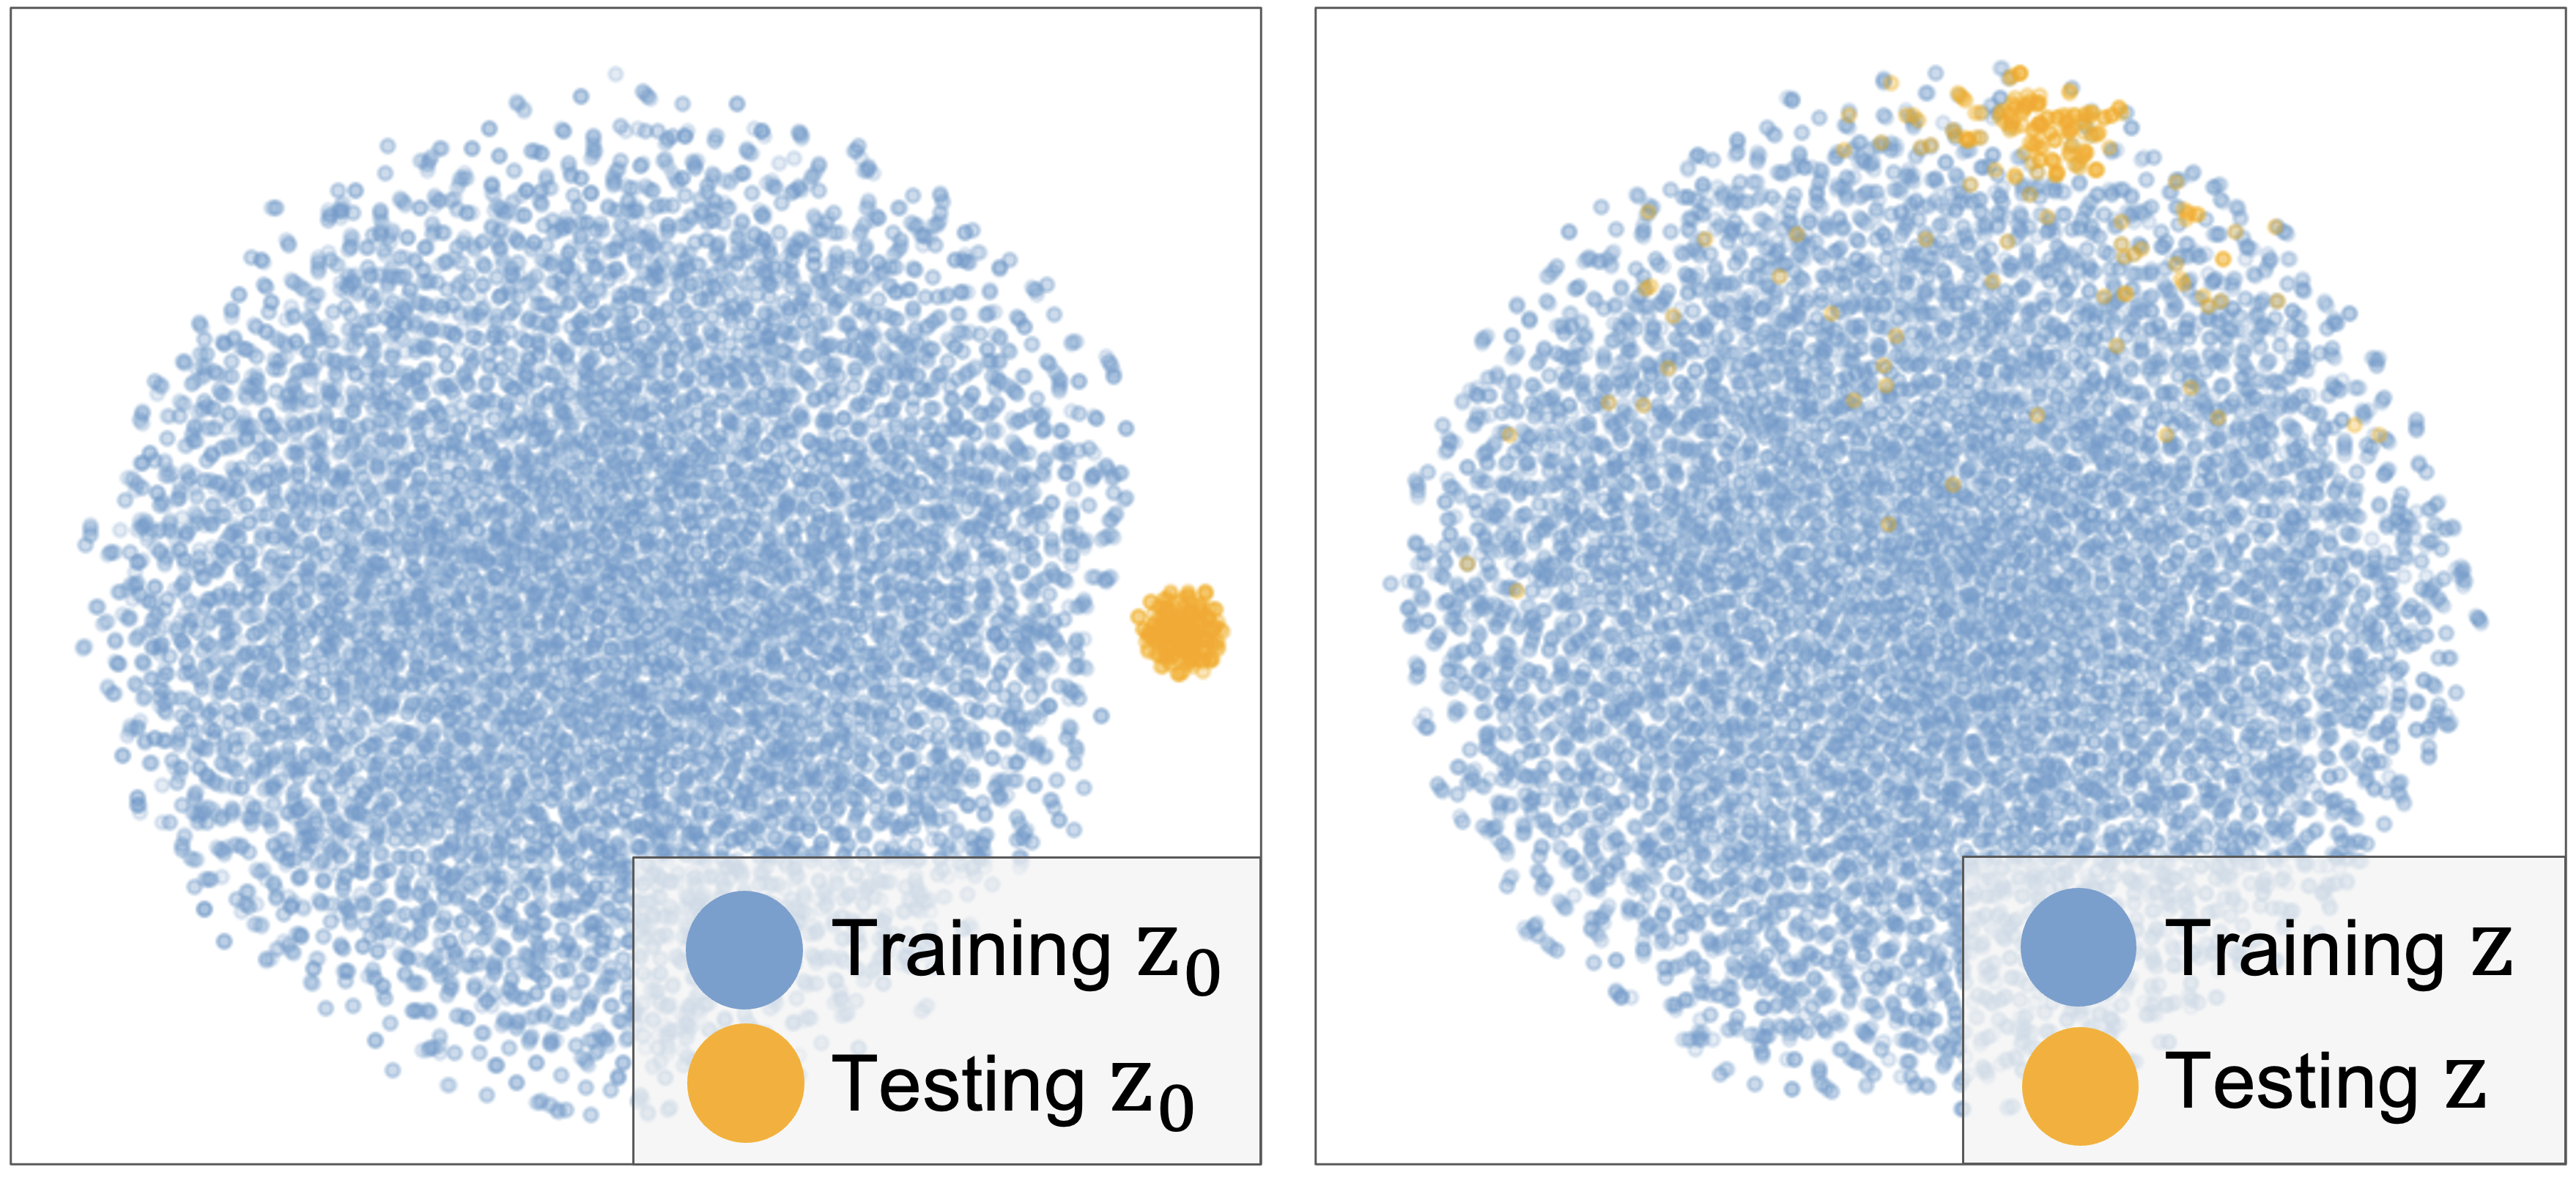
\includegraphics[width=\linewidth]{figures/tsne-all.png}
    \caption{t-SNE plot of latent variables in the Maze2D-medium. Left: Training $z_0$ from aggregated posterior $\E_{p_\mathcal{D}(\tau, y)}[p_\theta(z_0|\tau,y)]$. Testing $z_0$ from $p_\theta(z_0|y)$, disjoint from training population. Right: Distribution of $z=U_\alpha(z_0)$. }
    \label{fig:latent-tsne}
    \vspace{-2em}
\end{wrapfigure}


\cref{fig:maze2d_traj} visualizes samples from the training data and successful trajectories in testing. The left panels show that trajectories in training are suboptimal in terms of (1) being short in length and (2) containing very few goal-reaching instances. Trajectories on the right are generated by $10$ random runs with LPT, where the agent successfully navigates to the end goal from random starting positions in an effective manner. This indicates that the agent can discover the correlation between different $y$s to facilitate such stitching. 

To probe into the agent's understanding of trajectories' returns, we visualize the representation space of the latent variables. The left of \cref{fig:latent-tsne} is the aggregated posterior distribution of $z_0$. We can see that $z_0$ infered from $p_\theta(z_0|y)$ are distant away from the training population. The agent understands they are not very likely in the training set. The right of \cref{fig:latent-tsne} is the distribution of $z$, which is transformed from $z_0$ with the UNet, $z=U_\alpha(z_0)$. We observe that $z$s from the generated trajectories become ``in-distribution'' in the sense that some of them are mingled into the training population and the remaining lie inside a region coverable through linear interpolation of training samples. The agent understands what trajectories to generate even if they are unlikely among what it has seen. 




\subsection{Environment contingencies} 

To live in a stochastic world, contingent planning that is adaptable to unforeseen noises is desirable. \citet{paster2022you, yang2022dichotomy} discover that DT's performance would degrade in stochastic environments due to inevitable overfitting towards contingencies. We examine LPT and other baselines in Connect Four from~\citet{paster2022you}. Connect Four is a two-player game, where the opponent will make adversarial moves to deliberately disturb an agent's plan. According to the empirical study from~\citet{paster2022you}, the degradation of DT is more significant than in stochastic Gym tasks from~\citet{yang2022dichotomy}. As shown in Table \ref{table:connect4}, LPT achieves the highest score with minimal variance. The ESPER baseline is from~\citet{paster2022you}, which is very relevant to LPT as it is also a latent variable model. ESPER learns the latent variable model with an adversarial loss. It further adds a clustering loss in the latent space. LPT's on-par performance may justify that MLE upon a more flexible prior can play an equal role. 

\begin{table}[h]
% \vspace{-1.5em}
\centering
\caption{Evaluation results on Connect Four. \textbf{Bold} highlighting indicates top scores.}
\label{table:connect4}
\resizebox{0.65\linewidth}{!}{%
\centering
\begin{tabular}{lccccc}
\toprule
{Dataset}  &\multicolumn{1}{c}{CQL} & \multicolumn{1}{c}{DT} &\multicolumn{1}{c}{ESPER} &\multicolumn{1}{c}{LPT}\\
\midrule
Connect Four  &{$0.61\pm0.05$} &$0.8\pm0.07$ &$\mathbf{0.99}\pm0.03$ &$\mathbf{0.99}\pm0.01$\\
\bottomrule
% \bottomrule
\end{tabular}
}
\end{table}
\section{Limitations and Conclusion}
\label{sec:conclusion} 
\vspace{-0.2cm}
In this work, we studied various action space adapters (\asas) across a variety of embodiments, action spaces, and environments. We provide a generalization of prior works through the lens of action space adaptors, and for both discrete and continuous action spaces demonstrate designs that we show can leverage the knowledge within the \vlm.
Our findings conclude that for continuous actions, it is best to learn action tokens that accurately model the action distribution, while for discrete actions, it is best to reason over semantic language descriptions of actions.
We verify these ideas across \taskcount embodied AI tasks in 5 diverse environments.

A limitation of our work is all our analysis is under a single \vlm (\llava). Another limitation is that \rvq, the best performing \asa in continuous action spaces, requires collecting demonstrations to train the VQ model. Our analyses are also under only a single LoRA training setting. Future analyses can explore different base \vlms under different training regimes like full LLM finetuning. While our investigation of ASAs enables connecting a MLLM to various action spaces, the performance of these methods is still subpar for real-robot deployment where high success and safety are critical. MLLMs with the best ASA still struggle on simple environments like BabyAI, only achieving 40\% success rate. Further work is needed to improve the performance of these methods for real-world usage. Our investigation also only studies adapting MLLMs through behavioral cloning or on-policy RL. Future work can investigate if the choice of ASA varies when adapting the MLLM with other learning algorithms such as off-policy RL or offline RL.


{\small
\bibliographystyle{unsrtnat}
\setlength{\bibsep}{0pt}
\bibliography{main}
}

\newpage
\appendix
\section{Prior Work Comparison}
\label{sec:prior-work} 

In this section we expand on the differences between the prior work in action space adaptation mentioned in \Cref{sec:related-work} and our investigation. 
\Cref{table:prior-work} compares our investigation to prior work along several key dimensions. We emphasize that unlike prior works, ours studies a variety of action space adapters under a greater diversity of environments. 

\begin{table}
\resizebox{\columnwidth}{!}{
  \begin{tabular}{lp{6cm}p{3cm}p{5cm}llc}
    \toprule
    Work & Environments & Best \asa & Other \asas Studied & Action Space Types & Training & Using LLM/VLM? \\
    \midrule
    RoboFlamingo~\cite{li2023vision} & CALVIN & MLP & - & Continuous & BC & \greencheck \\
    Lamo~\cite{shi2023unleashing} & Franka Kitchen, Atari, MuJoCo & MLP & - & Continuous, Discrete & Offline-RL & \greencheck \\
    GFlan~\cite{carta2023grounding} & BabyAI & Sem Lang (scoring) & - & Discrete & Online RL & \greencheck \\
    RT-2~\cite{brohan2023rt} & Internal & Uniform & - & Continuous & BC & \greencheck \\
    LLaRP~\cite{szot2023large} & Language Rearrangement & MLP & - & Discrete & Online-RL & \greencheck \\
    VQ-BeT~\cite{lee2024behavior} & PushT, Multimodal Ant, BlockPush, Franka Kitchen, nuScenes, PlayKitchen & RVQ+MLP & - & Continuous & BC & \redx \\
    Ours & Language Rearrangement, Baby AI, MetaWorld, CALVIN, Habitat Skills & RVQ/ Sem-Lang & MLP, VQ, Uniform, Non-Sem, Non-Sem Comp &Continuous, Discrete & Online-RL, BC & \greencheck \\
    \bottomrule \\
  \end{tabular} 
}
\caption{
  Comparing our investigation to prior work. 
  Prior work typically analyzes a single action adapter in a single environment. 
  We study a variety of action adapters across a variety of environments. 
}
\label{table:prior-work} 
\end{table}

\subsection{Empirical Comparison to Prior Work}
\label{sec:prior-work-exp} 
We report performance on standard benchmarks which prior work has also extensively studied. However, even within the benchmarks there are differences in training algorithms and sensor input assumptions that make direct comparison to prior work difficult. Regardless of these differences, we study different \asas for \vlms in a consistent experimental setting. We also describe differences between the empirical setups of ours and prior works that perform well on these benchmarks.

\textbf{\metaworld} (\vlm+\rvq 84\% success rate on ML-45): To the best of our knowledge, our $ 84\%$ is the highest reported on \metaworld ML-45 so far. \citet{anand2021procedural} operates under similar sensor assumptions and achieves $ 77\%$ success with MuZero~\cite{schrittwieser2020mastering}. DualMind~\cite{wei2023imitation} achieves $ 79\%$ success rate on ML-45 and outperforms other generalist agents like Gato~\cite{reed2022generalist}. However, DualMind uses privileged simulator information about the joint states and object positions while we only use RGB visual observations.

\textbf{\calvin} (\vlm+\rvq 72\% success rate): RoboFlamingo achieves a higher $ 82\%$ success rate on the same $ ABC \rightarrow D$ task. However, RoboFlamingo uses the OpenFlamingo VLM while we use \llava. RoboFlamingo use the gripper and fixed camera while we only use the fixed camera. 
More recent work like 3D Diffuser Actor~\cite{ke20243d} practically solves the $ ABC \rightarrow D$ task, achieving $ 96 \%$ success rate. However, this work uses depth inputs, and a diffusion model policy that predicts keypoints for the end-effector rather than underlying actions. 
Our work uses only RGB visuals, uses a \vlm policy and predicts relative end-effector poses rather than keypoints.

\textbf{\langR} (\semlang 51\% success rate): This outperforms the prior highest reported number of $ 42 \%$ on the overall evaluation set from LLaRP~\cite{szot2023large}. 

\textbf{BabyAI} (\semlang 40\% success rate): GFlan~\cite{carta2023grounding} achieves $ 55\%$ success on the same evaluation split. However, the GFlan policy takes as input a ground truth language description of the state, while our policies take as input a $ 200\times 200$ RGB top down rendering of the environment. GFlan also trains the policy with reinforcement learning while we train with supervised learning. 

\begin{figure*}[!h]
  \centering
  \includegraphics[width=\textwidth]{figures/diagrams/envs.pdf}
  \caption{
    Visualizations of the environments we study. The top row shows an observation in the environment. The bottom row shows the associated instruction in that episode.
  }
  \label{fig:envs}
\end{figure*}

\section{Environment Details}
\label{sec:env-details}
An overview of the environments is visualized in \Cref{fig:envs}. This figure visualizes the training observations input to the agent. 
We run experiments on 5 environments, and each environment in turn consists of multiple tasks.
We arrive at the task count of \taskcount in the main paper through 45 tasks in \metaworld, 34 in \calvin, 20 in \habpick where we count each object goal as a different task, 10 in \langR for each of the evaluation splits, and 5 in BabyAI.
The task count for \langR is conservative since technically it consists of 282 instruction templates, each of which corresponds to a distinct task and goal.

\subsection{\metaworld}
\textbf{Tasks}: We use the ML-45 benchmark from \metaworld~\cite{metaworld}. Each of the 45 tasks are specified with a fixed language instruction. We use the task descriptions from Appendix Section A of \citet{metaworld}.

\textbf{Observation Space}: $ 200 \times 200$ RGB images from a fixed camera position. 
To render the visual observations, we only use the ``corner4" camera position as this gives an unobstructed view of the robot in most of the tasks. 

\textbf{Action Space}: 4DoF continuous control of the arm and gripper. The first 3 dimensions specify the relative end-effector translation. The last dimension specifies the desired gripper state.

\textbf{Training}: We use 40 start and goal configurations for each of the tasks. 
We generate 500 demonstrations for each of the 45 tasks. We use the scripted policies from~\citet{metaworld}. At each step we add Gaussian noise $ \mathcal{N}(0, 0.1)$ to the actions produced by the scripted policy before executing it in the environment.  We generate 500 successful trajectories per task, resulting in $ 45 \cdot 500 = 22.5k$ total trajectories.

\textbf{Evaluation}: We evaluate performance on 10 unseen start and goal configurations for each of the 45 tasks.
So in total, we evaluate on 450 unseen configurations and report the average performance over these 450 episodes.

\subsection{\calvin}
\textbf{Tasks}: We use the \calvin $ ABC \rightarrow D$ dataset split. 

\textbf{Observation Space}: $ 200 \times 200$ RGB observations from the fixed camera view. 

\textbf{Action Space}: 7DoF continuous control of the arm and gripper. The first 6 dimensions specify the relative position and rotation of the end-effector. The final dimension is a binary indicator for if the gripper should be open or closed.
We hold out $ 1024$ subsequences of the policy context length from these trajectories for reporting validation performance during the SFT process. 

\textbf{Training}: 
We use the 17,871 demonstrations provided in the CALVIN $ ABC \rightarrow D$ dataset. 
These demonstrations are in 3 different table backgrounds. 
This also includes 1,088 demonstrations for validation. 

\textbf{Evaluation}: 
We report performance on the $ D$ split. 
This evaluation scene is a different color than that encountered during training. 
All the start positions and goals are also different.
Many of the language instructions are also unseen from training.
We report the average performance over the 1,000 evaluation sequences. 
We report the success of the first task completed in the sequence.

\subsection{\Habpick}
\textbf{Tasks}: We use the same Pick task as in Habitat 2.0 Geometric Goal object rearrangement~\cite{szot2021habitat,habitatrearrangechallenge2022}, except we provide the agent the name of the object to rearrange rather than the starting coordinates of the object and increase the observation resolution. 
The task is successful when the agent picks up the object and returns the end-effector within a fixed offset to a ``resting position" in front of the robot.
The task ends in failure if the agent excessively collides with the scene, drops the object, or picks up the wrong object. 
The agent starts within 2 meters of the object and facing towards the receptacle but with random noise $ \mathcal{N}(0, 1.57)$ applied to the direction of facing directly at the receptacle.
The maximum number of steps per episode is 300 steps.

\textbf{Observation Space}: A $ 336 \times 336$ head-mounted RGB camera. 

\textbf{Action Space}: The action space is 10DoF control of the arm, base and gripper. The first 2 dimensions control the linear and angular velocity of the base. The next 7 dimensions control the relative joint offsets of the arm. The final dimension controls whether the suction gripper is engaged or not. 

\textbf{Training}: 
We first train a privileged policy with RL to complete the task. This policy takes as input the egocentric depth image and the ground truth position of the target object to pick up. We collect $ 20k$ successful trajectories.

\textbf{Evaluation}: 
We evaluate on the test episodes from \citet{habitatrearrangechallenge2022} which are $ 1,000$ episodes in unseen home layouts.

\subsection{BabyAI}
\textbf{Tasks}: 
The tasks all occur in a $ 6 \times 6$ grid populated with interactable objects. 
We use the task definitions from \citet{carta2023grounding}. This consists of the following 5 instruction templates: ``Go to $ <$object$>$", ``Pick up $<$object$>$", ``Put $<$object A$ >$ next to $ <$object B$>$,", ``Pick up $<$object A$>$ then go to $<$object B$>$ and Go to $<$object B$>$ after pick up $<$object A$>$", ``Unlock $<$door$>$". 
The maximum number of steps per episode is 50 steps.

\textbf{Observation Space}: $ 200 \times 200$ RGB observation as a top down of the $ 6 \times 6$ scene.
Note this is a more challenging observation space than prior gridworld navigation tasks that provide the current view as a compact entity specific array~\cite{babyai_iclr19} or by a language description~\cite{carta2023grounding}. 

\textbf{Action Space}: 
The action space consists of 6 actions consisting of: turn left, turn right, move forward, pick, drop and toggle. 

\textbf{Training}: 
We collect 1,000 demonstrations for each of the 5 templates. We randomly sample an instruction and starting state configuration for every demonstration. We use the expert planner from \citet{babyai_iclr19} to generate the demonstrations. 

\textbf{Evaluation}: 
We report performance on the unseen synonyms generalization test, described in Section 4.2 of \citet{carta2023grounding}.
We evaluate on 200 episodes per template type, giving 1000 total evaluation episodes.

\subsection{\LangR}
\textbf{Tasks}: An agent starts in an unseen house and must complete a rearrangement task from a language instruction. 

\textbf{Observation Space}: The agent has a $ 336 \times 336$ head-mounted RGB camera. We increase the camera resolution from $ 256 \times 256 $ in the original \langR task to match the input resolution of the \llava CLIP encoder.

\textbf{Action Space}: We use the same action space as from the original \langR benchmark \citet{szot2023large}. The agent can select between 70 high-level skills that include picking up objects by name, navigating to receptacles, placing on receptacles by name, and opening and closing receptacles by name.

\textbf{Training}: Since \langR does not provide any demonstrations and due to the emphasis on exploration in the problem, they are not readily obtainable, even with oracle planners. Therefore, we opt to train policies with reinforcement learning from the environment reward provided by the \langR task.

\textbf{Evaluation}: We evaluate on all 10 evaluation datasets from \langR consisting of 1,000 evaluation episodes on unseen scenes. 


\subsection{Task Groupings}
\label{sec:task-groupings} 
In \Cref{sec:experiments} we breakdown the performance on CALVIN and MetaWorld for task groupings. Each of the task groupings consists of multiple tasks from the benchmark. We grouped tasks in the following way:

\textbf{MetaWorld}: 
\begin{itemize}[itemsep=0pt,topsep=0pt,parsep=0pt,partopsep=0pt,parsep=0pt,leftmargin=*]
\item Articulated: ``door-close", ``door-open", ``drawer-close", ``drawer-open", ``faucet-open", ``faucet-close", ``handle-press-side", ``handle-press", ``window-open", ``window-close"
\item Press: ``button-press-topdown", ``button-press-topdown-wall", ``button-press", ``button-press-wall", ``coffee-button"
\item Push: ``plate-slide", ``plate-slide-side", ``plate-slide-back", ``plate-slide-back-side", ``push-back", ``push", ``push-wall", ``stick-push", ``sweep-into", ``sweep", ``soccer", ``coffee-push"
\item Pick: ``assembly", ``basketball", ``dial-turn", ``disassemble", ``hammer", ``peg-insert-side", ``peg-unplug-side", ``pick-out-of-hole", ``pick-place", ``pick-place-wall", ``reach", ``reach-wall", ``shelf-place"
\item Pull: ``coffee-pull", ``handle-pull-side", ``handle-pull", ``lever-pull", ``stick-pull"
\end{itemize}

\textbf{CALVIN}: 
\begin{itemize}[itemsep=0pt,topsep=0pt,parsep=0pt,partopsep=0pt,parsep=0pt,leftmargin=*]
\item Articulated: ``move slider left", ``open drawer", ``close drawer", ``move slider right"
\item Press: ``turn off led", ``turn on led", ``turn on lightbulb", ``turn off lightbulb"
\item Lift: ``lift blue block slider", ``lift pink block table", ``lift red block slider", ``lift red block table", ``lift pink block slider", ``lift blue block table"
\item Push: ``push pink block right", ``push blue block right", ``push red block left", ``push pink block left", ``push red block right", ``push blue block left", ``push into drawer"
\item Rotate: ``rotate red block right", ``rotate red block left", ``rotate pink block left", ``rotate pink block right", ``rotate blue block right", ``rotate blue block left"
\end{itemize}

\section{Further Policy Details}
\label{sec:method-details} 

\subsection{Prompt Details}


In addition to inputting the task instruction to the LLM, we also format the instruction with a prompt. We base our prompt off the prompt used in \llava. For all continuous control tasks, we use the prompt template ``Prompt: control the robot. USER: $<$INSTRUCTION$>$ ASSISTANT: ". 
For discrete action space tasks, we describe the available actions to the agent in the prompt as well. For BabyAI, this is the prompt template ``Prompt: Control the red triangle to complete the instruction using left, right, forward, pick, drop and toggle. USER: $<$INSTRUCTION$>$ ASSISTANT: ". For \langR, this is the prompt template ``Prompt: You are a home robot assistant. Your possible actions are: pick object, place receptacle, nav receptacle, open receptacle, close receptacle, STOP. - Objects: ball, clamp, hammer, screwdriver, padlock, scissors, block, drill, spatula, knife, spoon, plate, sponge, cleanser, plum, pear, peach, apple, lemon, can, box, banana, strawberry, lego, cube, book, bowl, cup, mug, orange, lid, toy, wrench. - Receptacles: chair, black table, brown table, TV stand, sink, right counter, left counter, sofa, fridge, left drawer, right drawer, middle drawer. USER: $<$INSTRUCTION$>$ ASSISTANT: ".



\subsection{Action Space Adapter Details}
\label{sec:asa-details} 

We use the same \asa details between all environments. We detail the architecture and training decisions for the different \asas when applicable. 

\textbf{\vq}: Use a codebook size of 512 with 512 dimensions per codebook element. 
These 512 tokens are mapped to token indices $ 31000-31512$ from the \llama language modeling head.
The encoder and decoder networks for predicting the latent and decoding from the latent are 4 layer MLP networks with hidden size 2048 using ReLU activations. The \vq network is trained on the actions in the same dataset used to train the policy. 
The network is trained with MSE loss to reconstruct the original actions. 
We \vq network for 3 epochs over the dataset.

\textbf{\rvq}: Use all the same details as \vq, but with a Residual-VQ that uses 2 codebooks. 

\textbf{\mlp}: We use a 2 layer MLP network with a hidden size of 2048 and ReLU activations. We use this same MLP network architecture for discrete and continuous action space tasks. In the robot manipulation tasks, we also found it useful to include the robot proprioception as input to the MLP network and included this as input to the network layer. The robot proprioception consists of the robot robot joint angles and the gripper state. This \asa requires no separate training. 

\textbf{\unif}: In the tasks we consider, the actions are already normalized to be in $ [-1,1]$. We then create $ 512$ evenly spaced bins within this interval and assign each action dimension based on which bin it is within. Like with \vq, we assign the 512 tokens to indices $ 31000-31512$ from the \llama language modeling head. This \asa requires no separate training.

\textbf{\lang}: Starting from the same semantic tokenization as with \semlang, we remap each token to the token corresponding to a digit ``0" to ``9". Therefore, the token count per action is the same between \lang and \semlang, but the \lang action tokens have no semantic meaning being just digits.

\subsection{Training and Architecture Details}
\label{sec:training-details} 
\label{sec:architecture-details} 
\label{sec:hyperparams} 

We use all pretrained components from \llava. For the visual token downsampler, we use a 2 layer Perceiver network~\cite{jaegle2021perceiver} with 4 output latents and hidden size 4096. 

We detail the hyperparameters used for imitation learning in in \Cref{table:hyperparams}. We trained with the HuggingFace Transformers library~\cite{wolf2019huggingface}, PyTorch~\cite{paszke2019pytorch}, DeepSpeed~\cite{rasley2020deepspeed}. 
For reinforcement learning, we use learning rate $ 3e^{-4}$, $ 32$ steps per rollout. $ 18$ parallel environment workers per GPU, an entropy coefficient of $ 0.01 $, 2 epochs over the data batch per rollout, 6 PPO minibatches, a maximum gradient norm of 0.2 and $ \gamma = 0.99$. 

We train the \calvin, \metaworld and \habpick imitation learning results on a 4xA40 GPU setup. We train the \langR and BabyAI experiments on a 8xA100-80GB GPU setup. 

We train the LLM weights with LoRA and fine tune the entire \asa and downsampler module. For LoRA we use rank value 128, alpha parameter $ 32$ and dropout $ 0.1$.


\begin{table}
\rowcolors{1}{white}{lightgray}
  \centering
  \begin{tabular}{r|cccc}
                       Hyperparameter &\calvin    & \metaworld&     BabyAI &\habpick \\
                        \hline \hline
                                   LR &$ 3e^{-4}$ & $ 3e^{-4}$& $ 3e^{-4}$ &$ 3e^{-4}$ \\
                            Optimizer &AdamW      &    AdamW  &      AdamW &AdamW \\
                     Number of Epochs &3          &      3    &         20 &20 \\
                   Batch Size Per GPU &32         &     32    &          8 &32 \\
                       Context Length &12         &      3    &         32 &3 \\
                       Max Gradient Norm & 1 & 1 & 1 & 1 \\

\end{tabular}

  \caption{
    Hyperparameters for all imitation learning experiments. Most hyperparameters are the same between environments but the number of training epochs, context length and batch size per GPU are adjusted to fit the need for history, environment dataset size and task complexity.
  }
  \label{table:hyperparams} 
\end{table}


\section{Qualitative Results}
See \Cref{fig:qual-results} for qualitative results of results from \Cref{fig:vlm-disc}. The \rvq \asa is visualized for Meta-World, CALVIN and Habitat Pick. \semlang is visualized for Language Rearrangement.

\begin{figure*}
    \centering
    \begin{subfigure}[t]{0.49\textwidth}
        \includegraphics[width=\textwidth]{figures/qual/mw_succ.jpg}
        \caption{The robot successfully picks the stick and pushes the box to the goal position.}
    \end{subfigure}
    \begin{subfigure}[t]{0.49\textwidth}
        \includegraphics[width=\textwidth]{figures/qual/mw_fail.jpg}
        \caption{The robot only partially lifts the handle and fails to lift it up all the way.}
    \end{subfigure}
    \begin{subfigure}[t]{0.49\textwidth}
        \includegraphics[width=\textwidth]{figures/qual/calvin_succ.jpg}
        \caption{The robot grasps the pink block and lifts it to the goal height.}
    \end{subfigure}
    \begin{subfigure}[t]{0.49\textwidth}
        \includegraphics[width=\textwidth]{figures/qual/calvin_fail.jpg}
        \caption{The robot attempts to grasp the blue block but grasps too high, failing to pick the block.}
    \end{subfigure}
    \begin{subfigure}[t]{0.49\textwidth}
        \includegraphics[width=\textwidth]{figures/qual/hab_succ.jpg}
        \caption{The robot moves closer to the cleaner bottle with its base and moves the arm to grasp the cleaner. It then returns the end-effector to the resting position to successfully end the task.}
    \end{subfigure}
    \begin{subfigure}[t]{0.49\textwidth}
        \includegraphics[width=\textwidth]{figures/qual/hab_fail.jpg}
        \caption{The robot correctly finds the lemon in the sink, but the tight sink receptacle results in the arm colliding with the sink and the episode terminating due to excessive collisions.}
    \end{subfigure}
    \begin{subfigure}[t]{0.49\textwidth}
        \includegraphics[width=\textwidth]{figures/qual/lang_succ.jpg}
        \caption{The robot searches the house, eventually finds the mug and then brings it to the blue table.}
    \end{subfigure}
    \begin{subfigure}[t]{0.49\textwidth}
        \includegraphics[width=\textwidth]{figures/qual/lang_fail.jpg}
        \caption{The robot picks the strawberry navigates to the counter area, but puts the strawberry on the right counter as opposed to the correct receptacle of the sink.}
    \end{subfigure}
    \caption{
        Qualitative visualizations of successes and failures from the results in Figure 1 of the main paper. The RVQ action space adapter is visualized for Meta-World, CALVIN and Habitat Pick. SemLang is visualized for Language Rearrangement.
    }
    \label{fig:qual-results} 
\end{figure*}

\section{Per-Task Breakdown}
\label{sec:per-task} 

In this section, we show results for each environment by task type. \Cref{table:langr_full_results} shows performance on Language Rearrangement for each of the evaluation datasets. \Cref{table:calvin-full} shows performance on \calvin for each of the \calvin tasks. \Cref{table:babyai-full} shows performance on BabyAI for each of the BabyAI instruction types. \Cref{table:metaworld-full} shows performance on \metaworld for each of the 45 \metaworld task types.

\begin{table}[h!] 
  \resizebox{\columnwidth}{!}{
      \begin{tabular}{l|ccc|ccccccccccc|}
        \toprule
        & \multicolumn{3}{c|}{Aggregated} & \multicolumn{11}{c|}{Per Dataset Breakdown} \\
        & \textbf{Total} & \textbf{Behavior} & \textbf{Paraphrastic} & \textbf{Train} & \textbf{Scene} & \textbf{Instruct} & \textbf{Novel} & \textbf{Multiple} & \textbf{Referring} & \textbf{Context} & \textbf{Irrelevant} & \textbf{Multiple} & \textbf{Spatial} & \textbf{Conditional} \\
        & & \textbf{Generalization} & \textbf{Robustness} & & & \textbf{Rephrasing} & \textbf{Objects} & \textbf{Rearrange} & \textbf{Expressions} & & \textbf{Text} & \textbf{Objects} & & \textbf{Instructs} \\
        \midrule \midrule
        \textbf{\semlang} &  51 {\scriptsize $ \pm$ 1  } &  56 {\scriptsize $ \pm$ 2  } &  47 {\scriptsize $ \pm$ 1  } &  94 {\scriptsize $ \pm$ 3  } &  94 {\scriptsize $ \pm$ 6  } &  92 {\scriptsize $ \pm$ 1  } &  97 {\scriptsize $ \pm$ 0  } &  80 {\scriptsize $ \pm$ 6  } &  31 {\scriptsize $ \pm$ 3  } &  46 {\scriptsize $ \pm$ 14  } &  66 {\scriptsize $ \pm$ 6  } &  2 {\scriptsize $ \pm$ 2  } &  0 {\scriptsize $ \pm$ 0  } &  46 {\scriptsize $ \pm$ 4  } \\
\textbf{\lang} &  27 {\scriptsize $ \pm$ 12  } &  31 {\scriptsize $ \pm$ 14  } &  24 {\scriptsize $ \pm$ 10  } &  72 {\scriptsize $ \pm$ 13  } &  58 {\scriptsize $ \pm$ 11  } &  74 {\scriptsize $ \pm$ 12  } &  76 {\scriptsize $ \pm$ 29  } &  21 {\scriptsize $ \pm$ 10  } &  10 {\scriptsize $ \pm$ 12  } &  12 {\scriptsize $ \pm$ 11  } &  20 {\scriptsize $ \pm$ 13  } &  0 {\scriptsize $ \pm$ 0  } &  2 {\scriptsize $ \pm$ 3  } &  26 {\scriptsize $ \pm$ 16  } \\
\textbf{\mlp} &  42 {\scriptsize $ \pm$ 2  } &  45 {\scriptsize $ \pm$ 3  } &  38 {\scriptsize $ \pm$ 1  } &  99 {\scriptsize $ \pm$ 1  } &  96 {\scriptsize $ \pm$ 4  } &  92 {\scriptsize $ \pm$ 2  } &  95 {\scriptsize $ \pm$ 4  } &  47 {\scriptsize $ \pm$ 5  } &  26 {\scriptsize $ \pm$ 2  } &  34 {\scriptsize $ \pm$ 2  } &  32 {\scriptsize $ \pm$ 2  } &  0 {\scriptsize $ \pm$ 1  } &  8 {\scriptsize $ \pm$ 1  } &  39 {\scriptsize $ \pm$ 3  } \\
\midrule 
 
      \end{tabular}
  }
  \caption{
    Evaluation results at 20M steps of RL training for all results in Language Rearrangement. We show averages and standard deviations over 2 random seeds of full policy training.
  }
  \label{table:langr_full_results} 
\end{table}

\begin{table}[h!] 
  \centering
    \begin{tabular}{ccccc}
\toprule
 & \textbf{\rvq} & \textbf{\mlp} & \textbf{\vq} & \textbf{\unif} \\
\midrule
\textbf{CALVIN} &  72  &  68  &  56  &  28  \\
\textbf{turn off led} &  50  &  96  &  36  &  16  \\
\textbf{move slider left} &  99  &  100  &  100  &  15  \\
\textbf{rotate red block right} &  54  &  17  &  35  &  17  \\
\textbf{open drawer} &  100  &  100  &  56  &  100  \\
\textbf{rotate red block left} &  31  &  14  &  14  &  14  \\
\textbf{push pink block right} &  31  &  100  &  51  &  14  \\
\textbf{push blue block right} &  42  &  27  &  35  &  20  \\
\textbf{push red block left} &  68  &  36  &  61  &  17  \\
\textbf{push pink block left} &  47  &  50  &  86  &  14  \\
\textbf{push red block right} &  35  &  35  &  17  &  17  \\
\textbf{push blue block left} &  56  &  27  &  47  &  14  \\
\textbf{push into drawer} &  49  &  34  &  14  &  14  \\
\textbf{rotate pink block left} &  76  &  73  &  73  &  16  \\
\textbf{turn on lightbulb} &  80  &  34  &  19  &  9  \\
\textbf{rotate pink block right} &  30  &  73  &  19  &  10  \\
\textbf{rotate blue block right} &  28  &  13  &  13  &  13  \\
\textbf{turn off lightbulb} &  76  &  19  &  19  &  12  \\
\textbf{lift blue block table} &  34  &  25  &  34  &  16  \\
\textbf{close drawer} &  100  &  100  &  100  &  70  \\
\textbf{rotate blue block left} &  32  &  11  &  38  &  20  \\
\textbf{move slider right} &  100  &  100  &  100  &  19  \\
\textbf{turn on led} &  31  &  100  &  42  &  14  \\
\textbf{lift blue block slider} &  32  &  22  &  51  &  15  \\
\textbf{lift pink block table} &  66  &  68  &  82  &  11  \\
\textbf{lift red block slider} &  56  &  22  &  41  &  13  \\
\textbf{lift red block table} &  45  &  53  &  15  &  15  \\
\textbf{lift pink block slider} &  75  &  12  &  62  &  12  \\

\end{tabular}

  \caption{Breakdown on every \calvin task. Note there are not an equal proportion of all tasks in the evaluation dataset.}
  \label{table:calvin-full} 
\end{table}

\begin{table}[h!] 
  \centering
    \begin{tabular}{cccc}
\toprule
 & \textbf{\semlang} & \textbf{\lang} & \textbf{\mlp} \\
\midrule
\textbf{goto} &  90  &  90  &  75  \\
\textbf{pickup} &  60  &  35  &  35  \\
\textbf{open} &  26  &  7  &  21  \\
\textbf{putnext} &  8  &  5  &  7  \\
\textbf{pick up seq go to} &  21  &  12  &  22  \\

\end{tabular}

  \caption{Breakdown on every BabyAI task.}
  \label{table:babyai-full} 
\end{table}



\begin{table}[h!] 
  \centering
    \begin{tabular}{ccccc}
\toprule
 & \textbf{\rvq} & \textbf{\mlp} & \textbf{\vq} & \textbf{\unif} \\
\midrule
\textbf{Meta-World} &  84  &  61  &  58  &  75  \\
\textbf{assembly} &  100  &  70  &  10  &  60  \\
\textbf{basketball} &  90  &  70  &  60  &  100  \\
\textbf{button-press-topdown} &  100  &  90  &  40  &  100  \\
\textbf{button-press-topdown-wall} &  100  &  100  &  60  &  90  \\
\textbf{button-press} &  100  &  100  &  70  &  100  \\
\textbf{button-press-wall} &  100  &  100  &  100  &  100  \\
\textbf{coffee-button} &  100  &  100  &  100  &  100  \\
\textbf{coffee-pull} &  100  &  40  &  30  &  50  \\
\textbf{coffee-push} &  80  &  20  &  30  &  80  \\
\textbf{dial-turn} &  100  &  50  &  40  &  100  \\
\textbf{disassemble} &  60  &  30  &  30  &  50  \\
\textbf{door-close} &  100  &  100  &  100  &  100  \\
\textbf{door-open} &  100  &  100  &  100  &  100  \\
\textbf{drawer-close} &  100  &  100  &  100  &  100  \\
\textbf{drawer-open} &  100  &  100  &  60  &  100  \\
\textbf{faucet-open} &  100  &  100  &  100  &  100  \\
\textbf{faucet-close} &  100  &  90  &  100  &  60  \\
\textbf{hammer} &  100  &  40  &  50  &  20  \\
\textbf{handle-press-side} &  100  &  100  &  100  &  100  \\
\textbf{handle-press} &  100  &  100  &  90  &  100  \\
\textbf{handle-pull-side} &  40  &  10  &  10  &  10  \\
\textbf{handle-pull} &  70  &  20  &  50  &  30  \\
\textbf{lever-pull} &  60  &  40  &  50  &  40  \\
\textbf{peg-insert-side} &  60  &  70  &  0  &  40  \\
\textbf{peg-unplug-side} &  50  &  30  &  100  &  90  \\
\textbf{pick-out-of-hole} &  50  &  90  &  40  &  30  \\
\textbf{pick-place} &  80  &  20  &  40  &  60  \\
\textbf{pick-place-wall} &  80  &  20  &  40  &  30  \\
\textbf{plate-slide} &  100  &  60  &  40  &  100  \\
\textbf{plate-slide-side} &  100  &  100  &  100  &  90  \\
\textbf{plate-slide-back} &  100  &  90  &  10  &  100  \\
\textbf{plate-slide-back-side} &  100  &  20  &  100  &  100  \\
\textbf{push-back} &  50  &  30  &  20  &  20  \\
\textbf{push} &  60  &  20  &  70  &  90  \\
\textbf{push-wall} &  80  &  40  &  60  &  100  \\
\textbf{reach} &  30  &  20  &  10  &  70  \\
\textbf{reach-wall} &  80  &  80  &  80  &  70  \\
\textbf{shelf-place} &  50  &  20  &  10  &  10  \\
\textbf{soccer} &  40  &  0  &  60  &  40  \\
\textbf{stick-push} &  100  &  60  &  10  &  100  \\
\textbf{stick-pull} &  90  &  50  &  30  &  100  \\
\textbf{sweep-into} &  70  &  40  &  60  &  70  \\
\textbf{sweep} &  90  &  30  &  50  &  70  \\
\textbf{window-open} &  100  &  100  &  100  &  100  \\
\textbf{window-close} &  100  &  100  &  100  &  100  \\

\end{tabular}

  \caption{Breakdown on every \metaworld task.}
  \label{table:metaworld-full} 
\end{table}



\ifincludecontent
  \input{sections/checklist}
\fi




\end{document}
